\chapter{实验数据分析}\label{chap:Epxeriment}

本章首先介绍了微译器的实验环境,在添加指令翻译过程的调试环境。
然后展示了微译器在x86和RISC-V上的性能分析,
最后分析了实施的优化方案的效果。

\section{实验环境}

本课题在Gem5模拟器\cite{gem5OriginalPaper}上进行了实验,Gem5是一个广泛使用的开源计算机系统体系结构模拟器,
它具有如下特点:
\begin{itemize}
  \item 开源:Gem5是一个开源项目,每年都会有大量的开发者参与到Gem5的开发中并发布新的版本。
  过去12年间,有超过250名开发者参与到Gem5的开发中,提交了超过7500次的commit\cite{Gem5SimulatorVersion2020}。
  目前最新的版本是v23,也是本文使用的版本。
  \item 广泛使用:Gem5被广泛用于学术界和工业界,用于研究新的计算机体系结构,新的内存层次结构,新的缓存替换算法等。
  \item 周期精确:Gem5是一个周期精确的模拟器,可以模拟CPU的每一个周期,\cite{Butko2012AccuracyEO}表明Gem5与实际硬件的性能差距在5\%以内。
  \item 多架构支持:Gem5支持多种指令集架构,包括x86、RISC-V、ARM等,可以方便的进行不同架构的模拟,便于本课题的研究。
  \item 模块化:Gem5的设计是模块化的,分为CPU模块、缓存模块、内存模块等,可以方便的进行模块的替换和扩展。
  \item 高度可配置:Gem5在一次编译后,在动态运行时可以通过配置参数进行不同的配置,例如CPU类型、缓存大小等。
  \item 事件驱动:Gem5是一个事件驱动的模拟器,它将时间的流逝模拟为一系列离散事件,只有在事件发生时才会进行模拟。
  例如在模拟CPU时,只有在取指、译码、执行等事件发生时才会进行慢速模拟,其余时间Gem5会快速跳过,这样可以提高模拟器的效率。
\end{itemize}

Gem5有全系统模拟器和用户空间模拟器两种模式,全系统模拟器可以模拟整个计算机系统,包括CPU、内存、外设等,
用户空间模拟器只模拟用户空间的部分,不模拟内核和硬件,只模拟用户空间的指令执行\cite{gem5OriginalPaper}。
本课题使用\textbf{用户空间}模拟器进行实验,因为本课题主要关注用户态二进制翻译器优化,只翻译用户态的指令,不涉及内核态的指令。

为了和真实的硬件环境更加接近,本文使用了和真实硬件校准过的Intel Haswell x86处理器\cite{haswell_cpu}参数进行模拟,
\cite{akramValidationGem5Simulator2019}校准后的数据表明,Gem5模拟器和真实硬件的性能差距在6\%以内。
本文将这个参数作为\textbf{基准参数},然后在这个基准参数上进行微译器的实验。接下来的性能对比都是相对于这个基准参数进行的。

为了不引入额外的面积、功耗等开销,本文使用同样大小的翻译缓存\textbf{替换}了原有的指令缓存,这样可以保证硬件开销不变。
表\ref{tab:specifications}展示了Gem5的硬件参数。

% https://www.tablesgenerator.com/latex_tables
\begin{table}[ht]
  \centering
  \bicaption{\enspace Gem5硬件参数,其中指令缓存模式为Intel Haswell处理器参数; 翻译缓存模式为微译器参数。
        仅替换了前端的指令缓存,其余参数保持不变。}{\enspace Gem5 hardware parameters}
  \label{tab:specifications}
  \begin{tabular}{|c|ll|}
  \hline
  \multicolumn{1}{|l|}{}         & \multicolumn{1}{l|}{\textbf{翻译缓存模式}} & \textbf{指令缓存模式} \\ \hline
  \multirow{6}{*}{\textbf{处理器核}} & \multicolumn{1}{l|}{软件动静翻译+融合微码}           & 硬件译码 + RISC-V指令    \\ \cline{2-3} 
                                 & \multicolumn{2}{l|}{类型:乱序6发射处理器}                         \\ \cline{2-3} 
                                 & \multicolumn{2}{l|}{译码:每拍6条}                         \\ \cline{2-3} 
                                 & \multicolumn{2}{l|}{主频:3.4GHz}                         \\ \cline{2-3} 
                                 & \multicolumn{2}{l|}{分发:每拍6条微码}                         \\ \cline{2-3} 
                                 & \multicolumn{2}{l|}{发射队列:69条微码}                                 \\ \cline{2-3} 
                                 & \multicolumn{2}{l|}{分支预测:4096项的锦标赛算法}                            \\ \hline
  \multirow{5}{*}{\textbf{\begin{tabular}[c]{@{}c@{}}内存层次\end{tabular}}} &
                    \multicolumn{1}{l|}{
                    \begin{tabular}[c]{@{}l@{}}翻译缓存: 32KB,\\8路组相连,2拍延迟\end{tabular}} &
                    \begin{tabular}[c]{@{}l@{}}指令缓存: 32KB,\\8路组相连,2拍延迟\end{tabular} \\ \cline{2-3} 
                                 & \multicolumn{2}{l|}{数据缓存: 32KB,8路组相连,2拍延迟}                    \\ \cline{2-3} 
                                 & \multicolumn{2}{l|}{二级缓存: 256KB,8路组相连,12拍延迟}                \\ \cline{2-3} 
                                 & \multicolumn{2}{l|}{三级缓存: 8MB,16路组相连,36拍延迟}                 \\ \cline{2-3} 
                                 & \multicolumn{2}{l|}{内存: 4GB,DDR3-1600, 30ns延迟}                     \\ \hline
  \end{tabular}
  \end{table}

\section{测试程序}

本课题使用了Coremark,SPEC CPU 2000测试集作为测试程序。
Coremark 是一个小型的基准测试程序,主要用于测试嵌入式系统的性能,它包括了一些基本的计算、控制流、内存访问等操作,可以通过参数指定循环次数来控制运行时间。
SPEC CPU 2000测试集是一个通用的测试CPU性能的测试集,包括了12个整数测试程序和14个浮点测试程序,是一个较为完备的测试集,本机运行时间在几分钟量级。

由于Gem5模拟器性能开销较大,在使用用户态模拟、乱序处理器模型的配置下,相对于本机运行时间,Gem5平均慢1万倍,这意味着一个在本机上运行1秒的程序,在Gem5上需要运行3小时。
因此选择SPEC 2000 test测试集来缩短实验时间,
而Coremark测试集设置循环1000次来控制运行时间,
所有测试程序在Gem5模拟器上运行的时间均控制在几分钟到几小时之间,这样方便本文进行实验。

测试程序使用riscv64-linux-gnu-gcc交叉编译器编译到RISC-V架构上,gcc 版本为12.3,
编译参数均为\texttt{-O3 --static}静态编译,SPEC程序还有其默认的编译参数。

\section{调试环境}

为了保证整个微译器的正确性,需要好的测试集和调试环境。


对于测试集,本文使用了单元测试、集成测试、性能测试等多种测试手段,保证了翻译器的正确性。
单元测试用于测试软件端翻译器的正确性,集成测试用于测试微译器在运行小型测试程序时的正确性,性能测试用于测试微译器在运行大型测试程序时的性能。
\begin{itemize}
\item 单元测试: 选择了riscv-tests\cite{riscv-tests}和riscv-arch-tests\cite{riscv-arch-tests},两者均使用汇编语言编写,用于测试单条RISC-V指令能否正确翻译运行,
前者对RISC-V IMAFD每条指令均有10余个测试用例,后者能生成数百个整数指令的随机测试用例。
\item 集成测试: 使用了手写的C语言程序,用于测试微译器在运行小型测试程序时的正确性,例如能否正确的初始化栈信息、能否正确处理系统调用等。
\item 性能测试: 使用了Coremark和SPEC 2000 test测试集,用于测试微译器在运行大型测试程序时的性能。
\end{itemize}

如果测试程序出现了错误,可以通过调试环境来定位错误。
由于Gem5上无法直接运行GDB调试器,本课题通过打印指令执行信息、打印寄存器信息等方式来定位错误。
对于含有错误的微译器,需要和标准正确的Gem5模拟器进行对比,找出错误的原因。
标准正确的Gem5模拟器是指没有任何修改的、配置为RISC-V架构的Gem5模拟器,它能直接硬件译码运行RISC-V程序。
通过在Gem5模拟器上添加了打印所有整数、浮点寄存器信息的功能,当指令执行流比对不一致时,可以通过打印寄存器信息来定位错误。

% \section{微译器在x86上性能分析}

% 图\ref{img:ucache_ipc}展示了微译器在x86上SPEC 2017上的翻译运行结果,相对于未修改过的x86指令缓存模式进行了归一化。
% 可以看到,微译器在SPEC 2017上的性能接近于原生运行,平均性能为92.3\%,并且一大半的浮点型测试集的性能损失在1\%以内。

% \begin{figure}[!htbp]
%   \centering
%   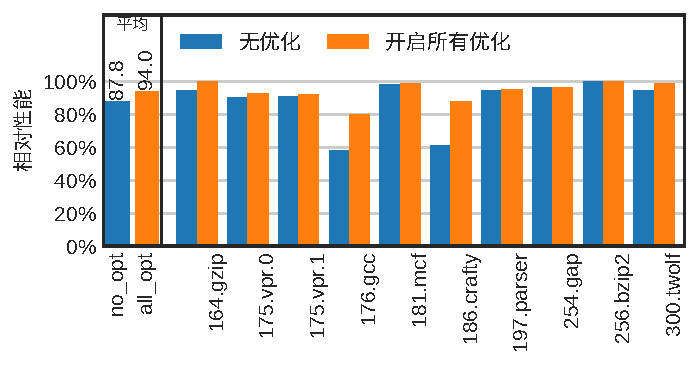
\includegraphics[width=1\linewidth]{./plot_pdf/ucache_ipc.pdf}
%   \caption{微译器运行SPEC CPU 2017的性能,相对于未修改过的x86指令缓存模式进行了归一化。}
%   \label{img:ucache_ipc}
% \end{figure}

% 图\ref{img:new_cache_miss}展示了微译器在x86上SPEC 2017上的每千条指令的未命中次数(MPKI),
% 根据计算,每千条指令的未命中次数和性能之间的皮尔森相关系数为-0.93,说明未命中次数和性能之间存在很强的负相关性。
% 这也说明了微译器的性能主要受到了未命中次数的影响。

% \begin{figure}[!htbp]
%   \centering
%   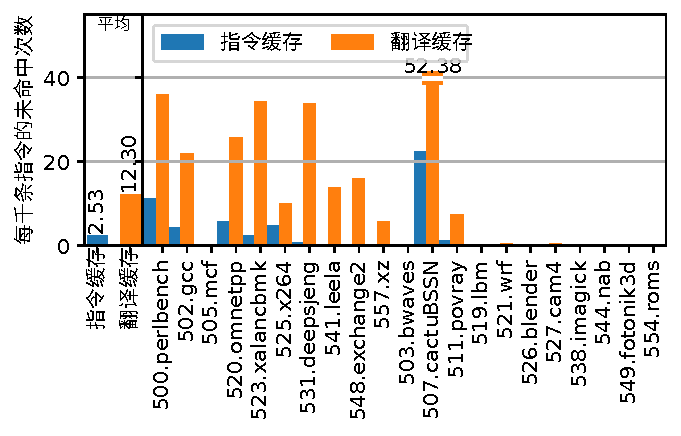
\includegraphics[width=1\linewidth]{./plot_pdf/new_cache_miss.pdf}
%   \caption{微译器运行SPEC CPU 2017的每千条指令的未命中次数。}
%   \label{img:new_cache_miss}
% \end{figure}

% \begin{table}[]
%   \centering
%   \caption{
%     微译器运行CoreMark测试集的性能对比。
%   }
%   \label{tab:coremark}
%   \begin{tabular}{llll}
%   \rowcolor[HTML]{FFCE93} 
%                & x86\_raw & x86\_ucache & riscv\_ucache \\
%   Insts        & 34655642 & 34655642    & 35899262      \\
%   Cycles       & 26220774 & 26301941    & 28797485      \\
%   IPC          & 1.321686 & 1.317608    & 1.246611      \\
%   IPC/IPC\_raw & 100\%    & 99.69\%     & 94.32\%      
%   \end{tabular}
%   \end{table}

% 本文在x86上运行了CoreMark测试集,相对于普通的ICache配置项,也就是没有任何修改的运行x86程序,
% 本文的微译器在翻译运行的性能为99\%,对应的每千条指令的未命中次数为0.9,也符合上述规律,
% 这主要在于程序的取指行为,CoreMark程序中主要为核心循环计算,时间局部性和空间局部性都很好,因此未命中次数较少,性能也较好。
% 即便经过微译器的预翻译文件膨胀,也能够在x86上保持较好的性能。

% 本文在RISC-V上运行了CoreMark测试集,得到了性能为94\%,对应的每千条指令的未命中次数为1.1,也符合上述规律。

% RISC-V 相对于x86的CoreMark 还有一定的性能差距,主要由于还没有添加硬件返回栈支持,导致对于函数调用的支持不够完善,因此性能有所下降。

% 同时RISC-V目前对于压缩指令支持还不够完善,导致翻译出来的微码编码较长,导致AOT文件相对更大,也会导致性能下降。


\section{性能分析}
由于Gem5的模拟器的性能开销较大,本文选择了SPEC CPU 2000 test测试集作为测试基准。
SPEC CPU 2000 test测试集包括了12个整数测试程序和14个浮点测试程序,是一个较为完备的测试集。
目前已经成功运行了8个整数测试程序,剩下的整数测试程序由于指令翻译的问题暂时无法运行,目前还在修复中,浮点测试程序还没有测试。

如图\ref{img:ipc}所示,本文的微译器在运行SPEC CPU 2000 test测试集时(这里只关注RISC-V程序),总共有三个测试配置,分别为:
\begin{itemize}
  \item 使用指令缓存(基准参数):CPU没有修改,通过内存层次、多级缓存和指令缓存,硬件译码并运行RISC-V程序。
  \item 使用翻译缓存:软件端二进制翻译器把RISC-V指令翻译为融合微码,CPU通过内存层次、多级缓存和微码缓存,硬件运行融合微码。
  \item 使用翻译缓存并有所有优化:在上一个配置基础上,开启了所有优化选项,让一行微码行中存储微码指令数目变多了,减少翻译缓存缺失率。
\end{itemize}

本文以指令每周期数(IPC)作为性能指标,IPC越大,性能越好。以指令缓存模式为基准性能,翻译缓存模式的性能为基准性能的百分比,
并分别测量关闭优化以及开启所有优化的性能。
如图\ref{img:ipc}所示,本文的微译器在运行SPEC2000 整数测试集时,性能表现如下:
在不开启任何优化的情况下,性能表现在加上微码缓存后,性能为原生性能87.8\%,其中主要是176.gcc和186.crafty两个测试程序性能下降较多;
这是由于这两个测试程序代码循环较少,时间局部性较差,指令代码较多,导致了大量的缓存缺失;
而对于其他的几个测试程序,性能大多在90\%以上,说明这些程序的时间局部性较好,性能下降较少,微译器的性能表现较好。

在开启所有优化后,性能为原生性能的94\%,性能提升了6\%,说明优化方案的效果较好。
对于176.gcc和186.crafty两个测试程序,性能提升较多,分别为20\%和24\%。
下一小节将对优化方案进行分析。


\begin{figure}[!htbp]
  \centering
  \includegraphics[width=0.8\linewidth]{./plot/ucache_ipc0.pdf}
  \bicaption{\enspace  SPEC2000整数性能对比图}{\enspace The performance comparison of SPEC2000 integer}
  \label{img:ipc}
\end{figure}

如图\ref{img:miss_rate}所示,本文的微译器在运行SPEC2000 整数测试集时,翻译缓存缺失率表现如下:
未开启优化时,缓存缺失率平均为2.3\%,其中最高的为gcc和crafty测试程序,缓存缺失率为7.7\%和9.2\%;这与性能表现相符,缓存缺失率越高,性能越低。
开启所有优化后,缓存缺失率平均为0.6\%,下降了1.7\%,说明优化方案的效果较好。
经过计算,缓存缺失率和性能之间的皮尔森相关系数为-0.91,说明缓存缺失率和性能之间存在很强的负相关性。目前的性能下降主要受到了未命中次数的影响。

\begin{figure}[!htbp]
  \centering
  \includegraphics[width=0.8\linewidth]{./plot/miss_rate.pdf}
  \bicaption{\enspace  SPEC2000整数测试下缓存缺失率}{\enspace The cache miss rate of SPEC2000 integer}
  \label{img:miss_rate}
\end{figure}

如图\ref{img:ipc_fp}所示,本文的微译器在运行SPEC2000 浮点测试集时,性能表现如下:
在不开启任何优化的情况下,性能表现在加上微码缓存后,性能为原生性能的96.5\%;
在开启所有优化后,性能为原生性能98.2\%,性能提升了1.7\%。
这说明无论是否开启优化,微译器对于浮点性能表现较好。


\begin{figure}[!htbp]
  \centering
  \includegraphics[width=0.8\linewidth]{./plot/ucacheipc_fp.pdf}
  \bicaption{\enspace  SPEC2000浮点性能对比图}{\enspace The performance comparison of SPEC2000 floating point}
  \label{img:ipc_fp}
\end{figure}


\section{优化方案分析}

本节将对第\ref{chap:Opt}章中提出的四种优化方案进行分析,分别是放松指令缓存行优化、放松条件跳转优化、添加压缩指令优化、使用变长微码缓存行优化。
由于Spec2000浮点测试在关闭和打开优化条件情况下,性能都接近原生性能,差异不大,因此这里不再分析。
后文将分析Spec2000\textbf{整数}测试集的优化效果。
为了防止不同优化条件相互影响,本文分别对每个优化方案单独进行分析,也就是单独开启其中一个优化方案,其余优化方案关闭。

\subsection{放松指令缓存行结尾优化}

\begin{figure}[!htbp]
  \centering
  \includegraphics[width=0.8\linewidth]{./plot/ucache_ipc1.pdf}
  \bicaption{\enspace  放松指令缓存行条件后性能对比图}{\enspace The performance comparison of relaxing instruction cache line}
  \label{img:ipc1}
\end{figure}

\begin{figure}[!htbp]
  \centering
  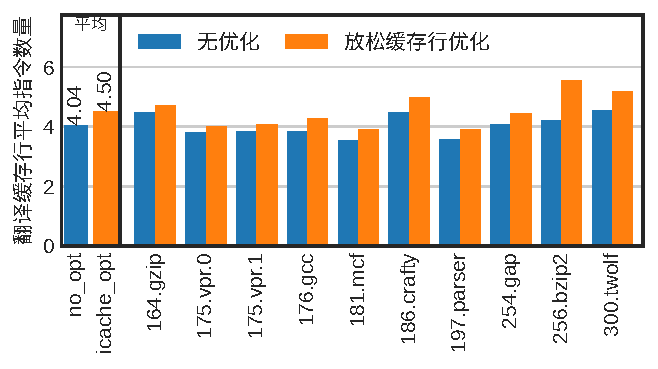
\includegraphics[width=0.8\linewidth]{./plot/ucacheline_nums1.pdf}
  \bicaption{\enspace  放松指令缓存行条件后翻译缓存行平均指令数量}{\enspace The average number of instructions in translation cache line after relaxing instruction cache line}
  \label{img:ucacheline_nums1}
\end{figure}

回顾第\ref{chap:Opt}章提出的优化方案1——放松指令缓存行结尾,也就是允许第二行的指令填充到上一行的翻译缓存行中,
这样相当于能提升上一行的翻译缓存行中的指令数量,等价于提升翻译缓存的有效容量,减少缓存缺失率,提升性能。

如图\ref{img:ipc1}所示,微译器在运行SPEC2000 整数测试集时,开启放松指令缓存行优化后,平均性能从87.8\%提升到了91.2\%,性能提升了3.4\%。
如图\ref{img:ucacheline_nums1}所示,开启放松指令缓存行优化后,翻译缓存行平均指令数量从4条提升到了4.5,提升了0.5条指令。
这说明放松指令缓存行优化方案有效提升了翻译缓存行的指令数量,减少了缓存缺失率,提升了性能。
但同样需要注意到,相对于64字节长的翻译缓存行,一行极限能存储12条指令,目前平均只存储了4.5条指令,还有较大的提升空间。

\subsection{放松条件跳转优化}

\begin{figure}[!htbp]
  \centering
  \includegraphics[width=0.8\linewidth]{./plot/ucache_ipc2.pdf}
  \bicaption{\enspace  放松条件跳转优化后性能对比图}{\enspace The performance comparison of relaxing conditional jump optimization}
  \label{img:ipc2}
\end{figure}

\begin{figure}[!htbp]
  \centering
  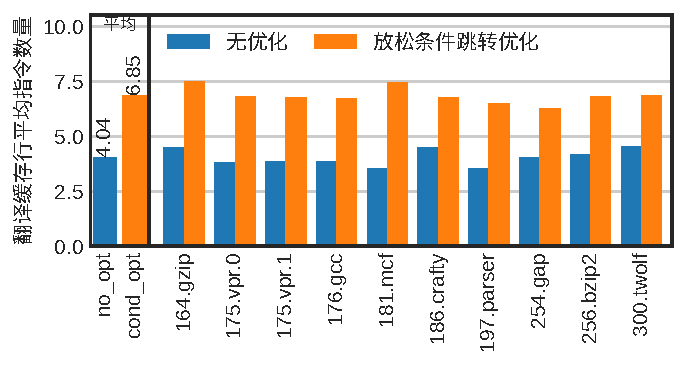
\includegraphics[width=0.8\linewidth]{./plot/ucacheline_nums2.pdf}
  \bicaption{\enspace  放松条件跳转后翻译缓存行平均指令数量}{\enspace The average number of instructions in translation cache line after relaxing conditional jump}
  \label{img:ucacheline_nums2}
\end{figure}

回顾第\ref{chap:Opt}章提出的优化方案2——放松条件跳转优化,也就是允许条件跳转指令后的指令仍然能放到同一行的翻译缓存行中,
这样对于不跳转的条件跳转指令,后续的指令仍然在同一行中,能继续执行。

如图\ref{img:ipc2}所示,微译器在运行SPEC2000 整数测试集时,开启放松条件跳转优化后,平均性能从87.8\%提升到了89.8\%,性能提升了2\%。
如图\ref{img:ucacheline_nums2}所示,开启放松条件跳转优化后,翻译缓存行平均指令数量从4条提升到了6.8条,提升了2.8条指令。
这说明放松条件跳转优化方案有效提升了翻译缓存行的指令数量,减少了缓存缺失率,提升了性能。
但平均指令数的提升大于性能的提升,说明条件跳转后的指令虽然放在了一行中,相当于分支预测静态预测一定不跳转,
但是如果实际跳转了,后续指令没有执行,也同样浪费了翻译缓存行的容量。



\subsection{压缩指令优化}

\begin{figure}[!htbp]
  \centering
  \includegraphics[width=0.8\linewidth]{./plot/ucache_ipc3.pdf}
  \bicaption{\enspace  添加压缩指令优化后性能对比图}{\enspace The performance comparison of adding compression instruction optimization}
  \label{img:ipc3}
\end{figure}

\begin{figure}[!htbp]
  \centering
  \includegraphics[width=0.8\linewidth]{./plot/tisa_avg_bytes.pdf}
  \bicaption{\enspace  添加压缩指令优化后平均指令长度变化}{\enspace The average instruction length change after adding compression instruction optimization}
  \label{img:avg_bytes}
\end{figure}

回顾第\ref{chap:Opt}章提出的优化方案3——添加压缩指令优化,也就是将融合微码指令压缩为更短的指令存储,减少翻译缓存行的占用。
如图\ref{img:ipc3}所示,微译器在运行SPEC2000 整数测试集时,开启压缩指令优化后,平均性能没有什么变化,性能为87.9\%。
如图\ref{img:avg_bytes}所示,开启压缩指令优化后,平均指令长度从4字节减少到了3.3字节,减少了0.7字节。
这说明压缩指令优化方案有效减少了融合指令平均指令长度,减少了翻译缓存行的占用,
但是由于翻译缓存行结束条件的限制,导致了翻译缓存行的指令数量没有增加,性能没有提升。
3.3字节的平均指令长度,也接近RISC-V C扩展压缩指令的平均长度(3字节),说明大部分RISC-V 压缩指令
都被翻译为融合微码的压缩指令,考虑到融合微码压缩指令同时支持x86指令的翻译,这个长度是可以接受的。

\subsection{变长微码缓存行优化}

\begin{figure}[!htbp]
  \centering
  \includegraphics[width=0.8\linewidth]{./plot/ucache_ipc4.pdf}
  \bicaption{\enspace  使用变长微码缓存行优化后性能对比图}{\enspace The performance comparison of using variable length microcode cache line optimization}
  \label{img:ipc4}
\end{figure}

回顾第\ref{chap:Opt}章提出的优化方案4——使用变长微码缓存行优化,也就是允许翻译缓存行的长度不固定,根据翻译缓存行的指令数量动态调整长度。
当指令数多时候使用64字节的翻译缓存行,当指令数少时候使用32字节的翻译缓存行。

如图\ref{img:ipc4}所示,微译器在运行SPEC2000 整数测试集时,开启变长微码缓存行优化后,平均性能从87.8\%提升到了92.2\%,性能提升了4.4\%。
这也是所有优化中效果最好的一个优化方案。
根据分析发现缓存行平均指令数为4.0条,而32字节的翻译缓存行最大能存储6条标准融合指令,存储4条指令是足够的,大部分情况下不需要使用64字节的翻译缓存行。
更短的翻译缓存行长度,意味着更高的存储效率,减少了缓存缺失率,提升了性能。


\section{本章小结}

本章首先介绍了微译器的实验环境,也就是使用Gem5模拟器的配置方案;
接下来介绍了测试程序,包括Coremark和SPEC CPU 2000 test测试集;
进一步介绍了调试环境,包括单元测试、集成测试、性能测试等;
接下来对微译器在RISC-V上运行的性能进行了分析,包括性能对比、缓存缺失率分析等。
最后对本文提出的4个优化方案进行了分析,分别是放松指令缓存行结尾优化、放松条件跳转优化、添加压缩指令优化、使用变长微码缓存行优化。
得出结论,放松指令缓存行结尾优化和放松条件跳转优化对性能提升效果较好,压缩指令优化对性能提升效果不显著,变长微码缓存行优化对性能提升效果最好。